\chapter{状态空间模型}

\section{线性系统的状态空间描述}

\subsection{线性系统的状态空间描述}

\begin{definition}[状态与状态空间]
    完全地表征系统时间域行为的最小个数的内部变量组称为系统的状态。组成这个变量组的变量$x_1(t),x_2(t),\cdots,x_n(t)$称为系统的状态变量，其中，$t \geq t_0$，$t_0$为系统的初始时刻。由状态变量构成的列向量
    \begin{equation*}
        \bm{x}(t) = \left[
            \begin{array}{c}
                x_1(t) \\ x_2(t) \\ \vdots \\ x_n(t)\\
            \end{array}
        \right] \quad t \geq t_0
    \end{equation*}

    称为系统的状态向量，简称为状态。状态向量的取值的向量空间称为状态空间。
\end{definition}

对于以上的定义，有如下几点需要注意：
\begin{enumerate}
    \item “完全表征系统时间域的行为”是指给定状态变量的初值，以及系统的输入信号，则系统在$t \geq t_0$时间域上的运动行为完全确定
    \item 状态变量组的“最小数目”的含义为状态变量$x_1(t),x_2(t),\cdots,x_n(t)$是能够完全表征系统运动特性的变量的最小个数，减少变量个数将不能完全表征系统
    \item 考虑系统内部的各个变量，则$x_1(t),x_2(t),\cdots,x_n(t)$构成系统变量中线性无关的一个极大无关组。具有$n$维状态变量的全体就构成了实数域上的$n$维空间
\end{enumerate}

\begin{corollary}
    一个动态系统任意选取的两个状态变量组之间为线性非奇异变换的关系（基变换关系）
\end{corollary}

\begin{definition}[状态方程与输出方程]
    输入引起状态变化的过程写成状态变量的一阶微分方程组的形式，称为系统的状态方程，即：
    \begin{equation*}
        \begin{split}
            \dot{x_1} &= f_1(x_1,x_2,\cdots,x_n;u_1,u_2,\cdots,u_r;t) \\
            \vdots & \\
            \dot{x_n} &= f_n(x_1,x_2,\cdots,x_n;u_1,u_2,\cdots,u_r;t) \\
        \end{split}
    \end{equation*}

    其中，$t\geq t_0$。在引入向量表示的基础上，可以将状态方程表示为向量方程的形式
    \begin{equation*}
        \dot{\bm{x}} = \bm{f}(\bm{x},\bm{u},t) \quad t \geq t_0
    \end{equation*}

    其中
    \begin{equation*}
        \bm{x}(t) = \left[
            \begin{array}{c}
                x_1(t) \\ \vdots \\ x_n(t) 
            \end{array}
        \right]
        \quad
        \bm{u} = \left[
            \begin{array}{c}
                u_1 \\ \vdots \\ u_r
            \end{array}
        \right]
        \quad 
        \bm{f}(\bm{x},\bm{u},t) = \left[
            \begin{array}{c}
                f_1(\bm{x},\bm{u},t) \\ \vdots \\ f_n(\bm{x},\bm{u},t)
            \end{array}
        \right]
    \end{equation*}

    类似，状态和输入决定输出变化，可以用如下的输出方程表示，即：
        \begin{equation*}
        \begin{split}
            \dot{y_1} &= g_1(x_1,x_2,\cdots,x_n;u_1,u_2,\cdots,u_r;t) \\
            \vdots & \\
            \dot{y_m} &= g_m(x_1,x_2,\cdots,x_n;u_1,u_2,\cdots,u_r;t) \\
        \end{split}
    \end{equation*}

    或者表示成向量方程的形式
        \begin{equation*}
        \bm{y} = \bm{g}(\bm{x},\bm{u},t) 
    \end{equation*}

    其中
    \begin{equation*}
        \bm{y}(t) = \left[
            \begin{array}{c}
                y_1(t) \\ \vdots \\ y_m(t) 
            \end{array}
        \right]
        \quad
        \bm{u} = \left[
            \begin{array}{c}
                u_1 \\ \vdots \\ u_r
            \end{array}
        \right]
        \quad 
        \bm{g}(\bm{x},\bm{u},t) = \left[
            \begin{array}{c}
                g_1(\bm{x},\bm{u},t) \\ \vdots \\ g_m(\bm{x},\bm{u},t)
            \end{array}
        \right]
    \end{equation*}
\end{definition}

系统的状态空间描述由状态方程和输出方程所组成，联合写出，则为：
\begin{equation*}
    \begin{aligned}
        \dot{\bm{x}} &= \bm{f}(\bm{x},\bm{u},t) \quad t \geq t_0 \\ 
        \dot{\bm{y}} &= \bm{g}(\bm{x},\bm{u},t)   \\
    \end{aligned}
\end{equation*}

如果考察线性系统的连续动态过程，可以将上述两个方程写成如下形式：
\begin{equation*}
    \begin{aligned}
        \dot{\bm{x}} &= \bm{A}(t) \bm{x} + \bm{B}(t) \bm{u} \quad t \geq t_0 \\
        \bm{y} &= \bm{C}(t) \bm{x} + \bm{D}(t) \bm{u}
    \end{aligned}
\end{equation*}

如果考察线性定常系统，则上述两个方程还能进行简化：
\begin{equation*}
    \begin{aligned}
        \dot{\bm{x}} &= \bm{A} \bm{x} + \bm{B} \bm{u} \quad t \geq t_0 \\
        \bm{y} &= \bm{C} \bm{x} + \bm{D} \bm{u}
    \end{aligned}
\end{equation*}

\subsection{状态空间表达式的建立}
系统的状态空间描述一般可以从三个途径求得：
\begin{enumerate}
    \item 由系统方框图建立，即根据系统各个环节的实际连结，写出相应的状态空间表达式
    \item 从系统的物理或者化学机理出发推导
    \item 由描述系统运动过程的高阶微分方程予以演化得到
\end{enumerate}

\subsubsection{从系统方框图建立状态空间表达式}
\begin{example}
    系统方框图如图所示，输入为$u$，输出为$y$，求其状态空间表达式
    \begin{center}
        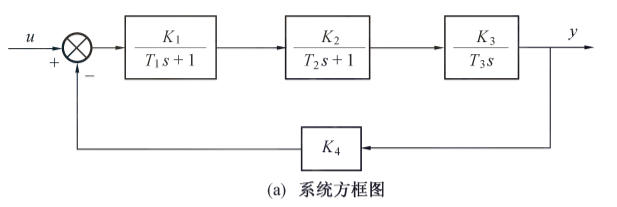
\includegraphics[width = 0.6\textwidth]{note/state space/figure/1.png}
    \end{center}

    \textbf{解}：各环节的模拟结构图下图所示：
    \begin{center}
        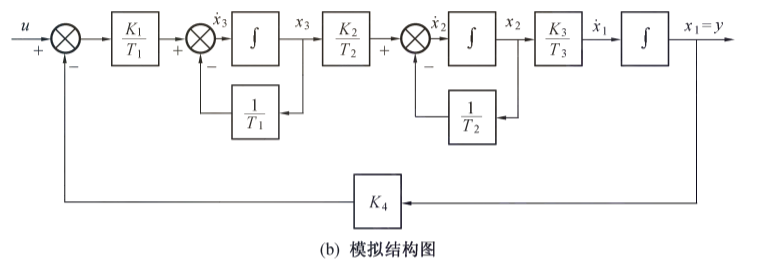
\includegraphics[width = 0.6\textwidth]{note/state space/figure/2.png}
    \end{center}

    由模拟结构图可以得到系统的状态方程为：
    \begin{equation*}
        \begin{aligned}
            \dot{x_1} &= \frac{K_3}{T_3} x_2 \\
            \dot{x_2} &= -\frac{1}{T_2} x_2 + \frac{K_2}{T_2} x_3 \\
            \dot{x_3} &= -\frac{1}{T_1}x_3 - \frac{K_1K_4}{T_1} x_1 + \frac{K_1}{T_1} u\\
        \end{aligned}
    \end{equation*}

    $y = x_1$ 为系统输出方程，写成向量和矩阵的形式，系统的状态空间表达式为：
    \begin{equation*}
        \begin{aligned}
            \dot{\bm{x}} &= \left[
                \begin{array}{ccc}
                    0 & \frac{K_3}{T_3} & 0 \\
                    0 & -\frac{1}{T_2} & \frac{K_2}{T_2} \\
                    -\frac{K_1K_4}{T_1} & 0 & -\frac{1}{T_1} \\
                \end{array}
            \right]
            \bm{x} + \left[
                \begin{array}{c}
                    0 \\ 0 \\ \frac{K_1}{T_1}
                \end{array}
            \right] u \\
            y &= \left[
                \begin{array}{ccc}
                    1 & 0 & 0\\
                \end{array}
            \right] \bm{x}
        \end{aligned}
    \end{equation*}
\end{example}

\subsubsection{从系统的机理出发建立状态空间表达式}
\begin{example}
    电网络如下图所示：输入量为电流源，输出变量取为电阻的输出电压，求此网络的状态空间表达式
    \begin{center}
        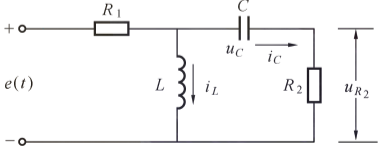
\includegraphics[width = .6\textwidth]{note/state space/figure/3.png}
    \end{center}

    \begin{enumerate}
        \item 确定状态变量，一般选取独立储能元件的线性无关变量作为状态变量。这里选取电容电压$u_C$和电感电流$i_L$作为电路的状态变量
        \item 列出电路方程：
        \begin{equation*}
            \begin{cases}
                R_1(i_C + i_L) + L \frac{di_L}{dt} = e(t) \\
                u_C + R_2 i_C = L \frac{di_L}{dt} \\
                i_C = C \frac{du_C}{dt}
            \end{cases}
        \end{equation*}
        \item 列写状态方程组和输出方程组。状态方程组为：
        \begin{equation*}
            \begin{cases}
                \frac{du_C}{dt} = - \frac{1}{(R_1+R_2)C}[u_C+R_1 i_L - e(t)]\\
                \frac{d i_L}{dt} = \frac{1}{L(R_1+R_2)}[R_1 u_C - R_1 R_2 i_L + R_2 e(t)]
            \end{cases}
        \end{equation*}

        输出方程为：
        \begin{equation*}
            u_{R_2} = R_2 i_C = R_2 C \frac{du_C}{dt} = -\frac{R_2}{R_1 + R_2}[u_C + R_1 i_L - e(t)]
        \end{equation*}

        \item 写成向量形式：
        \begin{equation*}
            \begin{split}
                &\left[
                    \begin{array}{c}
                        \frac{du_C}{dt} \\ \frac{di_L}{dt}
                    \end{array}
                \right] = 
                \left[
                    \begin{array}{cc}
                        -\frac{1}{(R_1 + R_2)C} & -\frac{R_1}{(R_1+R_2)C} \\
                        \frac{R_1}{L(R_1+R_2)} & -\frac{R_1 R_2}{L(R_1+R_2)}
                    \end{array}
                \right]
                \left[
                    \begin{array}{c}
                        u_C \\ i_L
                    \end{array}
                \right] + 
                \left[
                    \begin{array}{c}
                        \frac{1}{(R_1 + R_2)C} \\ \frac{R_2}{L(R_1+R_2)}
                    \end{array}
                \right]e(t) \\
                &u_{R_2} = \left[
                    \begin{array}{c}
                        -\frac{R_2}{R_1+R_2}
                    \end{array}
                \right]^T 
                \left[
                    \begin{array}{c}
                        u_C \\ i_L
                    \end{array}
                \right] + \frac{R_2}{R_1+R_2} e(t)
            \end{split}
        \end{equation*}
    \end{enumerate}
\end{example}

\subsubsection{由系统的输入输出传递关系求系统的状态空间描述}

\begin{enumerate}
    \item 化SISO系统输出描述为状态空间描述
    \begin{itemize}
        \item 由系统传递函数的部分分式展开求状态空间表达式

        将系统的传递函数部分分式展开为:
        \begin{equation*}
            G(s) = \frac{Y(s)}{U(s)} = \frac{\beta_{n-1} s^{n-1} + \cdots + \beta_1 s + \beta_0}{(s-\lambda_1)\cdots (s-\lambda_n)} = \sum^n_{i=1} \frac{c_i}{s-\lambda_i}
        \end{equation*}

        其中假设系统特征根互不相等，则

        \begin{equation*}
            Y(s) = \sum_{i=1}^n \frac{c_i}{s-\lambda_i} U(s)
        \end{equation*}

        令
        \begin{equation*}
            X_i(s) = \frac{U(s)}{s-\lambda_i}
        \end{equation*}

        则：
        \begin{equation*}
            s X_i(s) = \lambda_i X_i(s) = U(s)  \quad(i\leq n)
        \end{equation*}

        对上式进行laplace变换可得：
        \begin{equation*}
            \dot{x_i} = \lambda_i x_i + u
        \end{equation*}

        故系统的状态方程为：
        \begin{equation*}
            \left[
                \begin{array}{c}
                    \dot{x_1} \\ \dot{x_2} \\ \vdots \\ \dot{x_n}
                \end{array}
            \right] = diag(\lambda_1,\cdots,\lambda_n) 
            \left[
                \begin{array}{c}
                    x_1 \\ x_2 \\ \vdots \\ x_n
                \end{array}
            \right] + 
            \left[
                \begin{array}{c}
                    1\\ 1 \\ \vdots \\ 1
                \end{array}
            \right] u
        \end{equation*}

        输出方程为：
        \begin{equation*}
            y(t) = [c_1 \cdots c_n] \bm{x}
        \end{equation*}

        如果系统特征根中存在重根，以下用一个特殊的例子来说明：

        假设系统的传递函数为：
        \begin{center}
            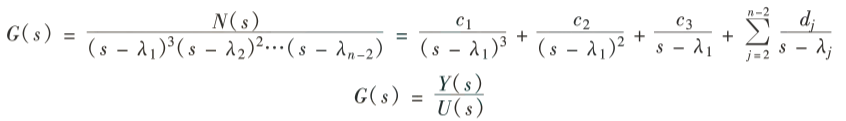
\includegraphics[width = .8\textwidth]{note/state space/figure/4.png}
        \end{center}

        此时有如下结果成立：
        \begin{center}
            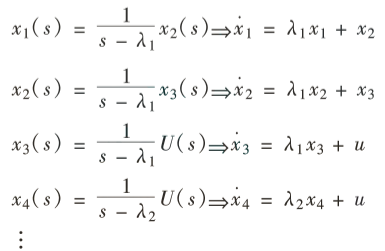
\includegraphics[width = .4\textwidth]{note/state space/figure/5.png}
        \end{center}

        可以写出系统状态方程如下：
        \begin{center}
            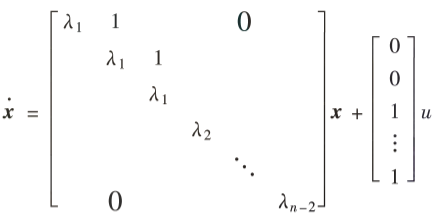
\includegraphics[width = .4\textwidth]{note/state space/figure/6.png}
        \end{center}

        系统输出方程如下：
        \begin{center}
            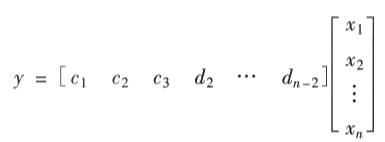
\includegraphics[width = .4\textwidth]{note/state space/figure/7.png}
        \end{center}

        \item 由高阶微分方程求状态空间表达式
        
        已知一个SISO系统，令y和u分别为其输出变量和输入变量，则输入输出间的动态关系可用一个高阶微分方程来表述，即：

        \begin{equation*}
            y^{(n)} + a_{n-1} y^{(n-1)} + \cdots + a_1 y^{(1)} + a_0 y = b_m u^{(m)} + b_{(m-1)} u^{(m-1)} + \cdots + b_1 u^{{1}} + b_0 u
        \end{equation*}

        假设系统初始条件为0，将上式两边进行Laplace变换，可得系统的传递函数：
        \begin{equation*}
            \frac{Y(s)}{U(s)} = \frac{b_m s^m + b_{m-1} s^{m-1} + \cdots +b_1 s +b_0}{s^n + a_{n-1} s^{n-1} + \cdots + a_1 s + a_0}
        \end{equation*}

        \begin{center}
            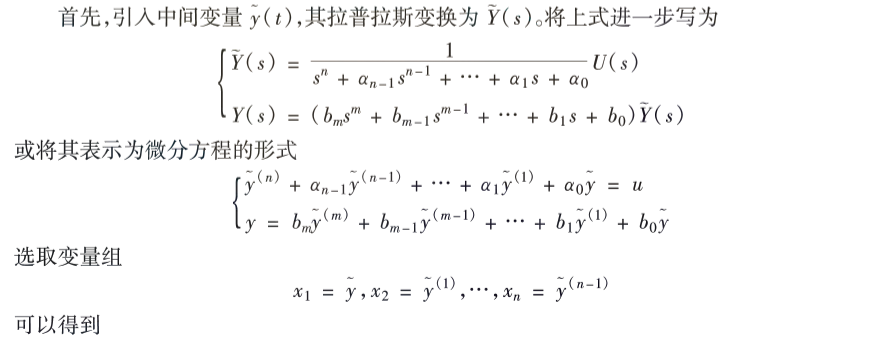
\includegraphics[width = .8\textwidth]{note/state space/figure/8.png}
        \end{center}

        \begin{center}
            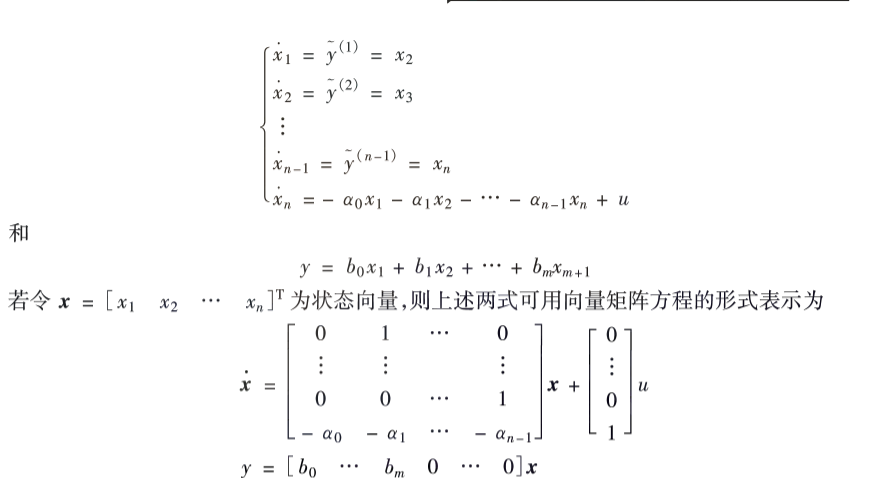
\includegraphics[width = .8\textwidth]{note/state space/figure/9.png}
        \end{center}
        
        如果该微分方程输出次数与输入相同，则传递函数可以拆成常数与一个分式之和，之后转化为上面的情况
    \end{itemize}

\end{enumerate}

\subsection{线性系统的代数等价}
\subsubsection{化状态空间为传递函数矩阵}

对于线性定常系统
\begin{equation*}
    \begin{cases}
        \dot{\bm{x}} = A \bm{x} + B \bm{u} \\
        \bm{y} = C \bm{x} + D \bm{u} 
    \end{cases}\quad t\geq t_0
\end{equation*}

对此式做Laplace变换，可导出
\begin{equation*}
    \begin{cases}
        s\bm{X}(s) = A \bm{X}(s) + B \bm{U}(s) \\
        \bm{Y} (s) = C \bm{X}(s) + D \bm{U}(s)  
    \end{cases}
    \Rightarrow 
    \begin{cases}
        \bm{X} (s) = (sI-A)^{-1} B\bm{U}(s) \\
        \bm{Y} (s) = [C (sI-A) ^{-1}B + D]U(s)
    \end{cases}
\end{equation*}

由此可以求出传递函数矩阵：
\begin{equation*}
    G(s) = C(sI - A)^{-1} B + D
\end{equation*}

\subsubsection{线性定常系统的几个概念}

\begin{definition}
    对于上述系统而言，称满足
    \begin{equation*}
        rank[sI-A \quad B] <n
    \end{equation*}

    的s为系统的输入解耦零点，称满足
    \begin{equation*}
        rank\left[
            \begin{array}{c}
                sI-A \\ C
            \end{array}
        \right]<n
    \end{equation*}

    的s为系统的输出解耦零点，称满足
    \begin{equation*}
        rank\left[
            \begin{array}{cc}
                sI-A & -B \\
                C & D \\
            \end{array}
        \right] <n + \min \{r,m\}
    \end{equation*}

    的s为系统的传输零点
\end{definition}

\subsubsection{代数等价系统}
\begin{definition}[代数等价]
    考虑两个同维数的线性定常系统：
    \begin{equation*}
        \begin{split}
            L:&\begin{cases}
                \dot{\bm{x}} = A \bm{x} + B \bm{u} \\
                    \bm{y} = C \bm{x} + D \bm{u} 
        \end{cases}\\
        L':&    \begin{cases}
        \dot{\overline{\bm{x}}} = \overline{A} \overline{\bm{x}} + \overline{B} \bm{u} \\
        \bm{\overline{y}} = \overline{C} \overline{\bm{x}} + \overline{D} \bm{u} 
    \end{cases}
        \end{split}
    \end{equation*}

    如果存在一个适当阶的定常可逆矩阵$P$，使得系统$L$和$L'$的系统参数矩阵满足：
    \begin{equation*}
        \overline{A} = PAP^{-1} \quad \overline{B} = PB \quad \overline{C} = CP^{-1} \quad \overline{D} = D
    \end{equation*}

    则称系统$L$和$L'$是代数等价的
\end{definition}

\subsubsection{代数等价系统的性质}

\begin{property}
    代数等价系统具有以下性质：
    \begin{enumerate}
        \item 相互代数等价的线性定常系统具有相同的特征方程、特征方程和极点
        \item 相互代数等价的线性定常系统具有相同的传递函数或传递函数矩阵
        \item 相互代数等价的线性定常系统具有相同的输入解耦零点、输出解耦零点和传输零点
    \end{enumerate}
\end{property}

\section{线性时变系统的运动分析}

\subsection{运动分析的含义}

\subsubsection{线性系统的运动分析与解存在唯一性}

对于线性时变系统，描述系统运动过程的状态方程为：
\begin{equation*}
    \dot{\bm{x}} = A(t) \bm{x} + B(t) \bm{u}  \quad   \bm{x}(t_0) = \bm{x}_0 \quad t \geq t_0
\end{equation*}

而对应的线性定常系统的状态方程为：
\begin{equation*}
    \dot{\bm{x}} = A \bm{x} + B \bm{u}  \quad   \bm{x}(0) = \bm{x}_0 \quad t \geq 0
\end{equation*}

显然，只有当状态方程满足初始条件的解存在唯一时，对系统的运动分析才是有意义的。这就要求状态方程中的系数矩阵和输入函数满足一定的假设，才可以保证方程解的存在唯一性。对于时变系统而言，如果系统矩阵$A(t)$和$B(t)$的所有的元素在时间定义区间$[t_0,t_f]$上均为实值连续函数，而输入$\bm{u}(t)$的元在时间区间$[t_0,t_f]$上是连续实函数，这时状态方程的解存在唯一

\subsubsection{线性系统响应的特点}

显然，线性系统的一个基本特征是其满足叠加原理。

自由运动是系统没有外部作用时：
\begin{equation*}
    \dot{\bm{x}} = A(t) \bm{x} \quad \bm{x}(t_0) = \bm{x}_0 \quad t \geq t_0
\end{equation*}
的解，用$\bm{\phi}(t,t_0,\bm{x}_0,0)$来表示，其中的$0$表示输入为零，称为零输入响应。强迫运动则是系统在零初始条件下的强迫方程
\begin{equation*}
    \dot{\bm{x}} = A(t) \bm{x} + B(t) \bm{u}  \quad   \bm{x}(t_0) =  \quad t \geq t_0
\end{equation*}
的解，用$\bm{\phi}(t,t_0,0,\bm{u})$来表示，称为零状态响应。系统由初始状态和输入作用所引起的整体响应$\bm{\phi}(t,t_0,\bm{x}_0,\bm{u})$就是两者的叠加，即：
\begin{equation*}
    \bm{\phi}(t,t_0,\bm{x}_0,\bm{u}) = \bm{\phi}(t,t_0,0,\bm{u}) + \bm{\phi}(t,t_0,\bm{x}_0,0)
\end{equation*}
这样，线性系统的运动分析可以分为两部分进行，然后再进行叠加


\section{线性定常系统的分析}
\subsection{线性定常系统的响应}
考察上述系统的状态转移矩阵。由于系统矩阵为定常矩阵$A$，显然满足条件式，于是系统的状态转移矩阵具有如下形式：
\begin{equation*}
    \bm{\Phi}(t,t_0) = I +\int_{t_0}^t A(\tau) d\tau + \frac{1}{2!}[\int_{t_0}^t A(\tau) d\tau]^2 + \cdots = e^{\int_{t_0}^t A(\tau) d\tau} = e^{A(t-t_0)}
\end{equation*}
当$t_0 = 0$时，$e^{At}$的表达式可以写为：
\begin{equation*}
    e^{At} = \sum_{k=0}^\infty \frac{1}{k!} A^k t^k
\end{equation*}
上式称为矩阵$A$的矩阵指数函数，即线性定常系统的状态转移矩阵为矩阵指数函数形式。

下面给出线性定常系统响应的结论：
\begin{theorem}
    给定线性定常系统，则有：
    \begin{enumerate}
        \item 其零输入响应为：
        \begin{equation*}
            \bm{\phi}(t,t_0,\bm{x}_0,0) = e^{A(t-t_0)} \bm{x}_0
        \end{equation*}
        \item 其零状态响应为：
        \begin{equation*}
            \bm{\phi}(t,t_0,0,\bm{u}) = \int_{t_0}^t e^{A(t-\tau)} B \bm{u}(\tau) d\tau
        \end{equation*}
        \item 其整体的状态响应为：
        \begin{equation*}
            \bm{\phi}(t,t_0,\bm{x}_0,\bm{u}) = e^{A(t-t_0)} \bm{x}_0 + \int_{t_0}^t e^{A(t-\tau)} B \bm{u}(\tau) d\tau
        \end{equation*}
    \end{enumerate}
\end{theorem}

\subsection{矩阵指数函数}
\subsubsection{矩阵指数函数的性质}
矩阵指数函数满足以下性质：
\begin{enumerate}
    \item $e^{A0} = I$
    \item $\frac{d}{dt} e^{At} = A e^{At}$
    \item $e^{A(t+s)} = e^{At} e^{As}$
    \item $(e^{At})^{-1} = e^{-At}$
    \item 当矩阵$A,B$可交换时：$e^{(A+B)t} = e^{At} e^{Bt} = e^{Bt} e^{At}$
    \item 若矩阵$P$为可逆矩阵，且$A = PJP^{-1}$，则$e^{At} = P e^{Jt} P^{-1}$
\end{enumerate}
\subsubsection{矩阵指数函数的求取}

\noindent \textbf{1}根据定义用级数来求取

\noindent \textbf{2}基于约当分解求取

这种方法的基本思想是先对矩阵$A$进行约当分解，然后利用性质6求取$e^{At}$

首先设$A$具有互异特征值$\lambda_i,i=1,2\cdots,n$，$\bm{p}_i$为$A$的与$\lambda_i$相对应的特征向量，记
\begin{equation*}
    P = [\bm{p}_1 \quad \bm{p}_2 \quad \cdots \quad \bm{p}_n]
\end{equation*}
则：
\begin{equation*}
    e^{At} = P \text{diag}(e^{\lambda_1 t} \quad e^{\lambda_2 t} \quad \cdots e^{\lambda_3 t}) P^{-1}
\end{equation*}
一般情况下，矩阵$A$的约当分解为：
\begin{equation*}
    A = P \text{diag}[J_1\quad J_2 \quad \cdots J_l] P^{-1}
\end{equation*}
其中$J_i$为约当块，此时有：
\begin{equation*}
    e^{At} = P \text{diag}(e^{J_1 t} \quad e^{J_2 t} \quad \cdots e^{J_3 t}) P^{-1}
\end{equation*}
再结合以下命题即可求解$e^{At}$
\begin{proposition}
    设$J_i$为一$p_i$阶约当块，$\lambda_i$为其特征值，其形式为：
    \begin{center}
        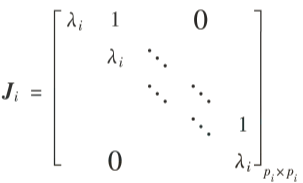
\includegraphics[width = .3\textwidth]{note/state space/figure/13.png}
    \end{center}
    则：
    \begin{center}
        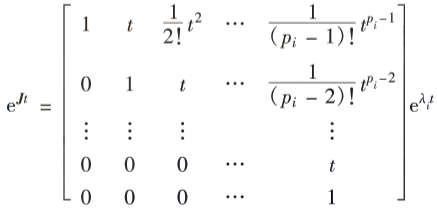
\includegraphics[width = .4\textwidth]{note/state space/figure/14.png}
    \end{center}
\end{proposition}

\noindent \textbf{3}利用Laplace变换求$e^{At}$
\begin{equation*}
    e^{At} = \mathcal{L}^{-1}[(sI - A)^{-1}]
\end{equation*}

证明从略

\noindent \textbf{4} 利用Cayley-Hamilton定理计算$e^{At}$

首先，先介绍一下Cayley-Hamilton定理
\begin{theorem}
    设$n$阶方阵$A$的特征方程为：
    \begin{equation*}
        f(\lambda) = \lambda^n + a_{n-1} s^{n-1} + \cdots + a_0 = 0
    \end{equation*}

    则方阵$A$满足$f(A) = 0$，即：
    \begin{equation*}
        A^n + a_{n-1} A^{n-1} + \cdots + a_0 = 0
    \end{equation*}
\end{theorem}

通过Cayley-Hamilton定理我们可以得到以下的结论：
\begin{center}
    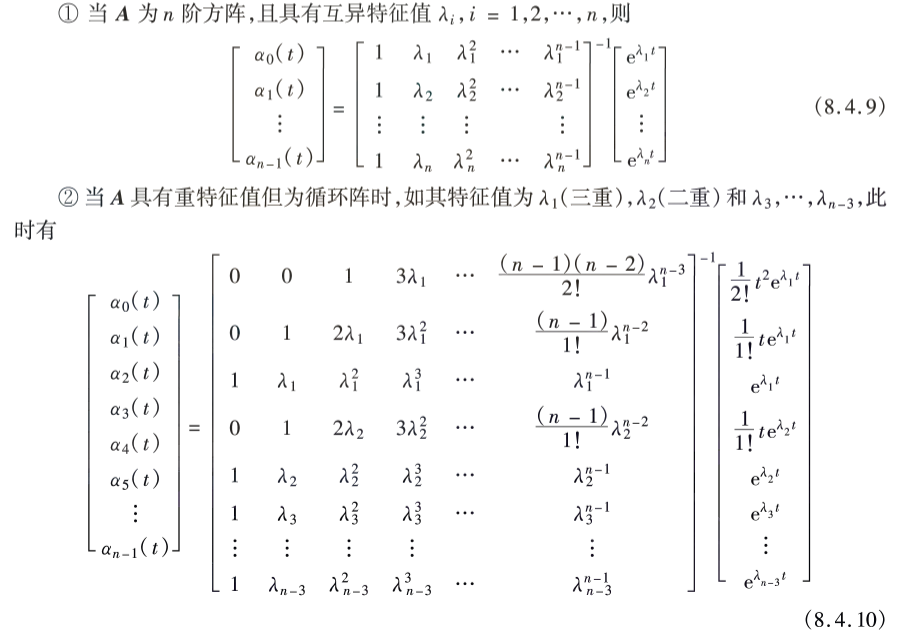
\includegraphics[width = \textwidth]{note/state space/figure/15.png}
\end{center}

\subsection{基于特征结构的状态响应表达}

假设系统矩阵$A$为$n$阶方阵，且其特征根两两相异：$\lambda_i \,(i=1,2,\cdots,n)$，假设每一个$\lambda_i$所对应的右特征向量为$v_i$，左特征向量为$w_i^T$，即：
\begin{equation*}
    A v_i = \lambda_i v_i \quad w_i^T A = w_i^T \lambda_i
\end{equation*}
则我们可以写出关于$A$的右特征向量矩阵与左特征向量矩阵：
\begin{equation*}
    P = [v_1,v_2,\cdots,v_n] \quad T = [w_1,w_2,\cdots,w_n]^T
\end{equation*}
则此时有以下两个式子成立：
\begin{equation*}
    \begin{split}
        e^{At} &= \sum_{i=1}^n v_i \overline{v_i}^T e^{\lambda_i t} \\
        &= \sum_{i=1}^n \overline{w_i} w_i^T e^{\lambda_i t}
    \end{split}
\end{equation*}
则此时我们可以写出这个表达式下的零输入响应与零状态响应：
\begin{equation*}
    \begin{split}
        x_{0u} = e^{At} x_0 &= \sum_{i=1}^n (v_i \overline{v_i}^T) x_0 e^{\lambda_i t} \\
        &= \sum_{i=1}^n (\overline{w_i} w_i^T) x_0 e^{\lambda_i t}
    \end{split}
\end{equation*}
\begin{equation*}
    \begin{split}
        x_{0x} &= \sum_{i=1}^n (v_i \overline{v_i}^T) \left[
            \sum_{j=1}^p b_j \int_0 ^t e^{\lambda_i (t-\tau)} u_j(\tau) d\tau
        \right]\\
        &= \sum_{i=1}^n (\overline{w_i} w_i^T) \left[
            \sum_{j=1}^p b_j \int_0 ^t e^{\lambda_i (t-\tau)} u_j(\tau) d\tau
        \right]
    \end{split}
\end{equation*}
其中$b_j$为B的第$j$列写状态方程组和输出方程组

\subsection{LTI系统的状态转移矩阵}

对于齐次状态方程，若有$x(t) = \Phi (t,t_0) x_0$，则称$\Phi(t,t_0)$为系统的状态转移矩阵。系统做自由运动时，它的运动形态唯一由状态转移矩阵决定，它包含了系统自由运动的全部信息

\begin{property}[状态转移矩阵的性质]
    \begin{enumerate}
        \item 状态转移矩阵的初始阵：$\Phi(0) = \Phi(t_0,t_0) = I$
        \item 状态转移矩阵的逆：$\Phi^{-1} (t,t_0) = \Phi(t_0,t)$
        \item 状态转移矩阵的传递性：$\Phi(t_2,t_1)\Phi(t_1,t_0) = \Phi(t_2,t_0)$
        \item 状态转移矩阵的导数：$\frac{d}{dt} \Phi(t,t_0) = A \Phi(t,t_0) = \Phi(t_0,t) A$
    \end{enumerate}
\end{property}

由上述信息可以写出系统状态响应与输出响应为：
\begin{equation*}
    \bm{x}(t) = \Phi(t,t_0)\bm{x}_0 + \int_{t_0}^t \Phi(t,\tau) B \bm{u}(\tau) d\tau
\end{equation*}
\begin{equation*}
    \bm{y}(t) = C \Phi(t,t_0) \bm{x}_0 +C \int_{t_0}^t \Phi(t,\tau) B \bm{u}(\tau) d\tau + D \bm{u}(t)
\end{equation*}

\section{离散系统状态空间分析}

\subsection{离散系统状态空间描述}

设线性离散系统的采样方式为周期采样，采样时刻为$kT,k\in N$，则状态空间描述为：
\begin{equation*}
    \begin{cases}
        \dot{\bm{x}}(k+1) = G(k)\bm{x}(k) + H(k) \bm{u}(k)\\
        \bm{y}(k) = C(k) \bm{x}(k) + D(k) \bm{u}(k)
    \end{cases}
\end{equation*}

其中$G,H,C,D$均为实矩阵，称$G(k)$为系统矩阵，$H(k)$为控制输入矩阵，$C(k)$为观测矩阵，$D(k)$为前馈矩阵。如果系统的参数矩阵均为定常的，即与采样时间标号$k$无关，则生疏式子可以化为以下式子：
\begin{equation*}
    \begin{cases}
        \dot{\bm{x}}(k+1) = G\bm{x}(k) + H \bm{u}(k)\\
        \bm{y}(k) = C \bm{x}(k) + D \bm{u}(k)
    \end{cases}
\end{equation*}

对于定常线性离散系统，我们称$G$的特征值为系统的特征值或极点。另外，类似于连续的情形，还有下述定义：
\begin{definition}
    对于上述线性定常离散系统，称满足
    \begin{equation*}
        rank[sI_n - G \quad H] < n
    \end{equation*}

    的$s$为系统的输入解耦零点，称满足
    \begin{equation*}
        rank \left[
            \begin{array}{c}
                sI_n - G \\    C
            \end{array}
        \right] <n
    \end{equation*}

    的$s$为系统的输出解耦零点，称满足
    \begin{equation*}
        rank \left[
            \begin{array}{cc}
                sI_n - G & -H \\
                C & D 
            \end{array}
        \right] < n+ min \{r,m\}
    \end{equation*}

    的s为系统的传输零点
\end{definition}

\subsubsection{离散系统状态空间的求法}

\noindent \textbf{1.}化差分方程为离散状态方程

这里假设差分方程中不含输入函数的高阶差分，即差分方程为：
\begin{equation*}
    y(k+n) + \sum_{i=1}^n a_i y(k+n-i) = b u(k)
\end{equation*}

选择状态变量为：
\begin{center}
    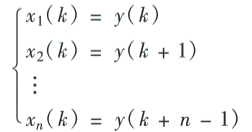
\includegraphics[width = .3\textwidth]{note/state space/figure/10.png}
\end{center}

则此时可以写出状态方程和输出方程为：
\begin{center}
    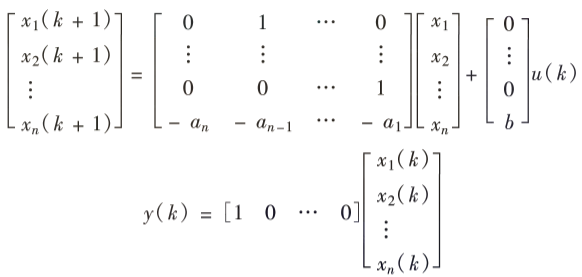
\includegraphics[width = .6\textwidth]{note/state space/figure/11.png}
\end{center}

\noindent \textbf{2.}化脉冲传递函数为离散状态方程

假设系统的脉冲传递函数$G(z)$分子分母多项式的阶数相同，且具有互不相同的实极点$z_1,\cdots,z_n$，则可以采用部分分式法将$G(z)$化为：
\begin{equation*}
    G(z) = \frac{\overline{y}(z)}{\overline{u}(z)} = d+ \sum_{i=1}^n \frac{k_i}{z-z_i}
\end{equation*}

上式中$\overline{y}(z),\overline{u}(z)$分别为输入输出的Z变换，$k_i = \text{Res}[G(z),z_i]$

取$\overline{x}_i(z) = \frac{1}{z-z_i} \overline{u}(z)$为离散状态变量的Z变换，则有：
\begin{equation*}
    z\overline{x}_i(z) = z_i \overline{x}_i(z) + \overline{u}(z)
\end{equation*}
\begin{equation*}
    \overline{y}(z) = d\overline{u}(z) + \sum_{i=1}^n k_i \overline{x}_i (z)
\end{equation*}

此时系统的状态方程和输出方程为：
\begin{center}
    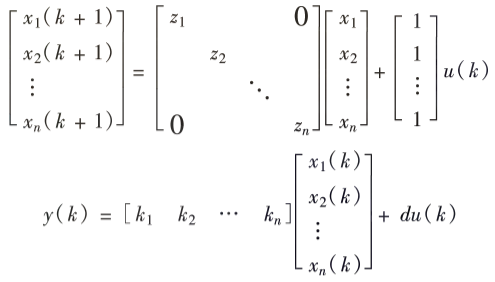
\includegraphics[width = .6\textwidth]{note/state space/figure/12.png}
\end{center}

\noindent \textbf{3.}线性连续系统状态方程的离散化

给定线性连续时变系统
\begin{equation*}
    \begin{cases}
        \dot{\bm{x}} = A(t) \bm{x} + B(t) \bm{u}  \quad t\in[t_0,t_a] \\
        \bm{y} = C(t) \bm{x} + D(t) \bm{u} \quad \bm{x}(t_0) = \bm{x}_0
    \end{cases}
\end{equation*}

则其离散化后的状态方程为：
\begin{equation*}
    \begin{cases}
        \bm{x}(k+1) = G(k) \bm{x}(k) + H(k) \bm{x}(k) \quad k = 0,1,\cdots,l \\
        \bm{y}(k) = C(k) \bm{x}(k) + D(k) \bm{u}(k) \quad \bm{x}(0) = \bm{x}_0
    \end{cases}
\end{equation*}

并且两者的系数矩阵间存在如下关系式：
\begin{equation*}
    \begin{split}
        G(k) &= \Phi[(k+1)T,kT] = \Phi(k+1,k) \\
        H(k) &= \int_{kT}^{(k+1)T} \Phi[(k+1)T,\tau]B(\tau) d\tau \\
        C(k) &= [C(t)]_{t=kT} \\
        D(k) &= [D(t)]_{t=kT} \\
    \end{split}
\end{equation*}

特别的，给定LTI系统
\begin{equation*}
    \begin{cases}
        \dot{\bm{x}} = A \bm{x} + B \bm{u} \quad \bm{x}(0) = \bm{x}_0 \\
        \bm{y} = C \bm{x} + D \bm{u}
    \end{cases}
\end{equation*}

的时间离散化模型可以写为：
\begin{equation*}
    \begin{cases}
        \bm{x}(k+1) = G \bm{x}(k) + H \bm{u}(k) \quad  \bm{x}(0) = \bm{x}_0 \\
        \bm{y}(k) = C \bm{x}(k) + D \bm{u}(k) \quad k = 0,1,2,\cdots
    \end{cases}
\end{equation*}

其中：
\begin{equation*}
    G = e^{AT} \qquad H = (\int_0^T e^{At} dt) B
\end{equation*}

这个系统的状态转移矩阵为：
\begin{equation*}
    \Phi(k) = G^k
\end{equation*}

\subsection{线性离散系统的运动分析}

\subsubsection{状态表达式的求解}

\noindent \textbf{1.}迭代法求状态表达式

对于上述提到的LTI系统而言，其状态运动的表达式为：
\begin{equation*}
    \bm{x}(k) = G^k \bm{x}_0 + \sum_{i=0}^{k-1} G^{k-i-1} H \bm{u}(i)
\end{equation*}

或
\begin{equation*}
    \bm{x}(k) = G^k \bm{x}_0 + \sum_{i=0}^{k-1} G^i H \bm{u}(k-i-1)
\end{equation*}

\noindent \textbf{2.}Z变换求状态表达式

对于上述LTI系统的状态差分方程而言，对其进行Z变换有：
\begin{equation*}
    z \bm{X}(z) - z\bm{x}_0 = G \bm{X}(z) + H \bm{U}(z)
\end{equation*}

故有：
\begin{equation*}
    \bm{x}(k) = Z^{-1}[\bm{X}(z)] = Z^{-1}[(zI - G)^{-1} (z \bm{x_0} + H \bm{U}(z))]
\end{equation*}

\subsubsection{状态转移矩阵的求法}

\noindent \textbf{1.}Z变换法

由上述两种求状态表达式的结果可以得到：
\begin{equation*}
    \Phi(k) = G^k = Z^{-1} [(zI - G )^{-1} z]
\end{equation*}

\noindent \textbf{2.}化矩阵$G$为标准型

首先讨论最特殊的情况：$G$的特征根没有重根

则此时我们可以取出其对应的右特征向量$P$，将$G$相似对角化为：
\begin{equation*}
    \varLambda = \text{diag}(\lambda_1,\lambda_2,\cdots,\lambda_n)
\end{equation*}

则此时我们可以求出状态转移矩阵为：
\begin{equation*}
    \Phi(k) = G^k = P \varLambda^k P^{-1} = P \text{diag}(\lambda_1^k,\lambda_2^k,\cdots,\lambda_n^k) P^{-1}
\end{equation*}

现在考虑$G$中特征根存在重根的情况，由于此时无法正常写出右特征向量矩阵，故此时将引入广义特征向量：
\begin{definition}[广义特征向量]
    矩阵$A$的广义特征向量满足：
    \begin{equation*}
        (A - \lambda I)^k v = 0 \quad k\geq 1
    \end{equation*}
    但：
    \begin{equation*}
        (A - \lambda I)^{k-1} v \neq 0 
    \end{equation*}
    广义特征向量可以组成一个向量链，设$\{P_1,P_2,\cdots,P_s\}$时对应于特征值$\lambda$的广义特征向量链，则这个向量链满足以下式子：
    \begin{equation*}
        \begin{cases}
            (A - \lambda I) P_1 = 0 \quad \text{（$P_1$是普通特征向量）}  \\
            (A - \lambda I) P_2 = P_1 \\
            (A - \lambda I) P_3 = P_2 \\
            \vdots \\
            (A - \lambda I) P_s = P_{s-1}
        \end{cases}
    \end{equation*}
\end{definition}

此时利用广义特征向量的定义，我们可以写出矩阵$G$的右特征向量矩阵$Q$，并将$G$化为其约旦标准型：

\begin{equation*}
    J = \text{diag}(J_1,J_2,\cdots,J_m)
\end{equation*}

此时我们可以写出状态转移矩阵为：
\begin{equation*}
    \Phi(k) = G^k = Q J^k Q^{-1} = Q \text{diag}(J_1^k,J_2^k,\cdots,J_m^k) Q^{-1}
\end{equation*}

其中$J_i$为特征值$\lambda_i$所对应的约旦块

\noindent \textbf{3.}化为关于G的有限项

由Cayley-Hamilton定理我们知道$G$一定为其特征方程的一个解，此时我们可以离散虚体部分状态转移矩阵写为$G$的有限项求和，即：
\begin{equation*}
    \Phi(k) = \sum_{i=0}^{n-1} \alpha_i(k) G^i
\end{equation*}

其中$\alpha_i(k)$为待定系数，可以仿照连续系统来求

\section{能控性与能观性}

在现代控制理论中,能控性和能观测性是两个重要的概念,它们是最优控制和最优估计的理论基础,基本的概念如下:
\begin{definition}[能控性与能观性的概念]
    \begin{itemize}
        \item 能控性是控制作用输入$u(t)$支配系统的状态向量$x(t)$的能力
        \item 能观测性是系统的输出$y(t)$反映系统的状态向量$x(t)$的能力
    \end{itemize}
    
    前者回答了$u(t)$能否使$x(t)$做任意转移的问题,后者则是回答了能否通过系统的输出量$y(t)$确定系统状态$x(t)$的问题
\end{definition}

\subsection{连续系统的能控性}

系统的能控性本质是在回答一个问题:已知某系统的当前时刻及其状态,是否存在一个容许控制,使得系统在该控制的作用下于有限时间后达到某个希望的特定状态?

由此,我们可以引出能控状态与系统的能控性的定义:
\begin{definition}[能控状态]
    对于线性定常系统,如果存在一个时刻$t_1 > 0$和一个无约束的容许控制$u(t),\quad t \in \left[0,t_1\right]$,使得系统在这个控制的作用下,系统由$x_0$出发经过时间$t_1$后由$x_0$转移到$x(t_1) = 0$,则称此$x_0$是系统的一个能控状态
\end{definition}

\begin{definition}[系统的能控性]
    对于线性定常系统,如果状态空间中的所有非零状态都是能控状态,则称该系统是能控的
\end{definition}

显然:时变系统的能控性和系统初始状态有关,而定常线性系统的能控性与初始时刻无关.

对于以上的定义,有几点需要注意:
\begin{enumerate}
    \item 能控性是一种定性性质,不涉及实现所需控制的具体方式
    \item 对定常系统,能控与否与$t_0$无关,与时间区间$\left[ t_0,t_1 \right]$无关,而对于时变系统,能控性与$t_0$和时间区间均有关
    \item 能控性只由系统的参数决定,因此是系统的固有属性
    \item 状态转移的轨迹没加以限制和规定,能控性是表征系统状态运动的一个定性特征
    \item 对线性定常系统能控性和能达性事等价的,但是对于时变系统和离散系统则是不等价的
    \item 不特殊说明,系统可控性均指状态能控性,要与输出能控性相区别
\end{enumerate}

在上面的注意事项中出现了能达性这个概念,我们现在来介绍这个概念:
\begin{definition}[能达状态]
    对于线性定常系统,如果存在一个时刻$t_1 > 0$和一个无约束的容许控制$u(t),\quad t \in \left[0,t_1\right]$,使得系统在这个控制的作用下,由零初始状态出发经过时间$t_1$后转移到$x(t_1) = x_f$,则称此$x_f$是系统的一个能达状态
\end{definition}

\begin{definition}[系统能达]
    对于线性定常系统,如果状态空间中的所有非零状态都是能达状态,则称此系统是能达的
\end{definition}

\subsection{系统能控性判据}

我们可以通过以下的几种方式判断下面的线性定常系统的能控性
\begin{equation*}
    \dot{x}(t) = A x(t) + B u(t)
\end{equation*}

上面的系统中$x$为$n$维状态向量;$u$为$r$维输入向量;$A \in \mathbb{R}^{n \times n}$和$B \in \mathbb{R}^{n \times r}$分别为系统矩阵和输入矩阵,均为常矩阵

\begin{theorem}
    线性定常系统是能控的当且仅当存在时刻$t_1 > 0$,使Gram矩阵
    \begin{equation*}
        W_c(t_1) = \int_0^{t_1} e^{-At} B B^T e^{-A^T t} dt 
    \end{equation*}
    是非奇异的
\end{theorem}

\begin{theorem}
    线性定常系统能控的充分必要条件是
    \begin{equation*}
        rank\left[\begin{array}{cccc}
            B & AB & \cdots & A^{n-1}B
        \end{array}\right] = n
    \end{equation*}
    其中$n = dim A$,我们称上述矩阵为$Q_c$
\end{theorem}

\begin{theorem}[PBH判据]
    线性定常系统是能控的当且仅当系统矩阵$A$的所有特征值$\lambda_i$满足:
    \begin{equation*}
        rank\left[ \lambda_i I - A \quad B \right] = n \quad \forall i \leq n
    \end{equation*}
    或者可以等价表述为:
    \begin{equation*}
        rank \left[ sI - A \quad B \right] = n \quad \forall s \in \mathbb{C}
    \end{equation*}
\end{theorem}

但是可能有些系统本身比较复杂，我们需要采用非奇异状态变换将这个系统化成一个比较简单的系统，可以通过以下的定理描述对于非奇异线性变换后的系统与原系统能控性之间的联系：

\begin{theorem}
    给定线性定常系统，通过非奇异状态变换$x = P \bar{x}$后的系统为$\dot{x} = \bar{A} \bar{x} + \bar{B} u$，则有：
    \begin{equation*}
        \text{rank}\left[
            \begin{array}{cccc}
                \bar{B} & \bar{A}\bar{B} & \cdots & \bar{A}^{n-1} \bar{B}
            \end{array}
        \right] = \text{rank} \left[
            \begin{array}{cccc}
                B & AB & \cdots & A^{n-1} B
            \end{array}
        \right]
    \end{equation*}
    其中$n$为系统状态变量的维数
\end{theorem}

我们还可以通过矩阵的Jordan标准型来判断系统的能控性：
\begin{theorem}
    \begin{center}
        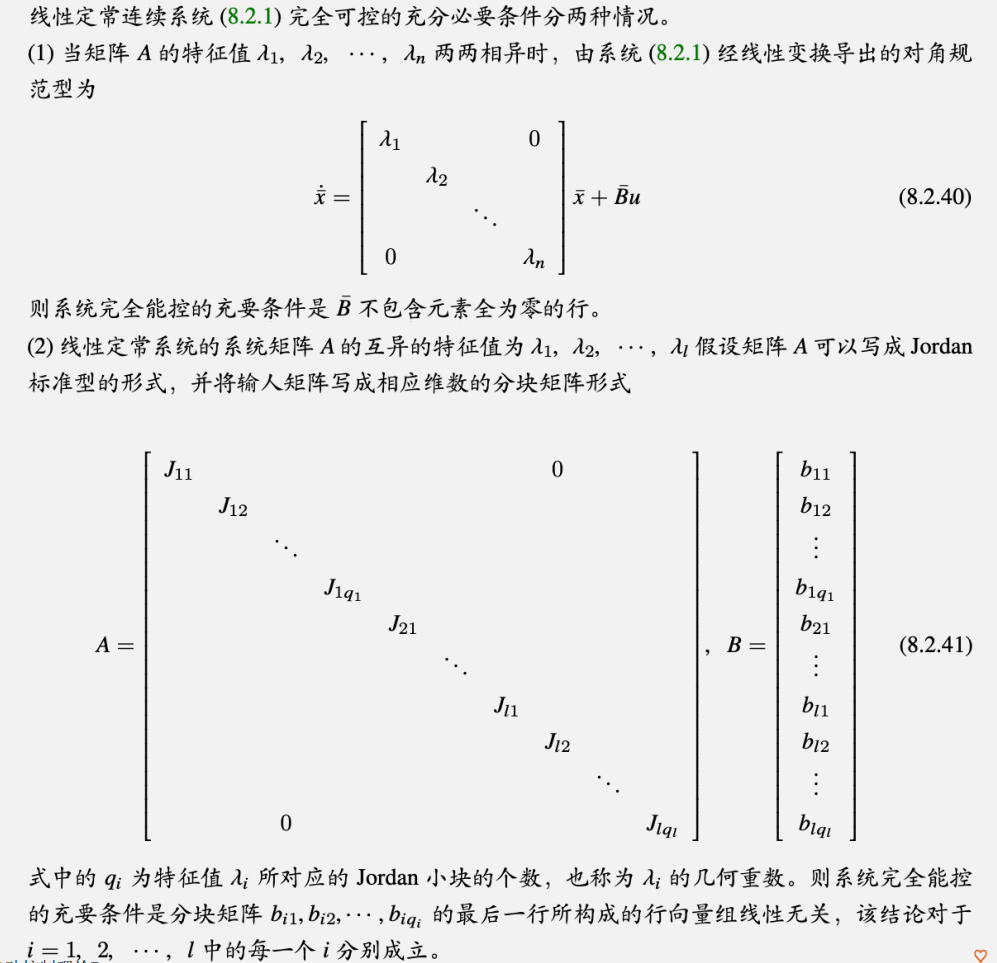
\includegraphics[width = .7\textwidth]{note/state space/figure/16.png}
    \end{center}
\end{theorem}

\subsection{连续系统的能观性}

和系统的能控性类似，我们可以给出系统能观性的概念：
\begin{definition}[能观状态]
    对于线性定常系统,如果对于初始时刻$t = 0$的一个非零初始状态$x_0$以及时间区间$\left[ 0,t_1 \right]$,使得由区间$[0,t_1]$上的系统输出$y(t)$可以唯一决定系统初始状态$x_0$,则称该状态$x_0$是能观的
\end{definition}

\begin{definition}[系统能观性]
    对于线性定常系统,如果状态空间中的所有非零状态都是能观状态,则称该系统是能观的
\end{definition}

同样的,时变系统的能观性依赖于初始时刻,而定长线性系统的能控性与能观性与初始时刻无关

\subsection{系统能观性判据}

我们可以通过以下的几种方式判断下面的线性定常系统的能观性:
\begin{equation*}
    \begin{split}
            \dot{x} &= A x\\
            y & = C x
    \end{split}
\end{equation*}

上面的系统中$x$为$n$维状态向量;$y$是$m$维输出向量;$A \in \mathbb{R}^{n \times n}$和$C \in \mathbb{R}^{m \times n}$分别为系统输入矩阵和系统输出矩阵,均为常矩阵

\begin{theorem}
    线性定常连续系统能观的充分必要条件是,存在有限时刻$t_1 > 0$,使Gram矩阵
    \begin{equation*}
        W_O(t_1) = \int_0^{t_1} e^{A^T t} C^T C e^{A t} dt
    \end{equation*}
    是非奇异的
\end{theorem}

\begin{theorem}
    线性定常系统能观的充分必要条件为:
    \begin{equation*}
        \text{rank} Q_O = \text{rank} \left[
            \begin{array}{c}
                C \\ CA \\ \vdots \\  C A^{n-1}
            \end{array}
        \right] = n
    \end{equation*}

    或者
    \begin{equation*}
        \text{rank} \left[
            \begin{array}{cccc}
                C^T & A^T C^T & \cdots & (A^T)^{n-1} C^T
            \end{array}
        \right] = n
    \end{equation*}
\end{theorem}

\begin{theorem}[PBH判据]
    线性定常系统完全能观的充分必要条件是,对矩阵$A$的所有特征值$\lambda_i,i \leq n$,均有:
    \begin{equation*}
        \text{rank}\left[
            \begin{array}{c}
                C \\ \lambda_i I - A
            \end{array}
        \right] = n
    \end{equation*}

    或者等价表述为:
    \begin{equation*}
        \text{rank} \left[
            \begin{array}{c}
                C \\ s I - A 
            \end{array}
        \right] = n \quad \forall s \in \mathbb{C}
    \end{equation*}
\end{theorem}

同样的，对于非奇异状态变换后的系统能观性与原系统能观性之间的联系，我们有以下的定理：
\begin{theorem}
    给定线性定常系统，通过非奇异状态变换$x = P \bar{x}$后的系统为
    \begin{equation*}
        \begin{split}
            \dot{x} &= \bar{A} x \\
            y &= \bar{C} x
        \end{split}
    \end{equation*}
    则有：
    \begin{equation*}
        \text{rank} \left[
            \begin{array}{c}
                \bar{C} \\ \bar{C} \bar{A} \\ \vdots \\ \bar{C} \bar{A}^{n-1}
            \end{array}
        \right] = \text{rank} \left[
            \begin{array}{c}
                C \\ C A \\ \vdots \\ C A^{n-1}
            \end{array}
        \right]
    \end{equation*}
    其中$n$为系统状态变量的维数
\end{theorem}

与能控性类似，也可以用系统的Jordan标准型来判断系统能观性：
\begin{theorem}
    \begin{center}
        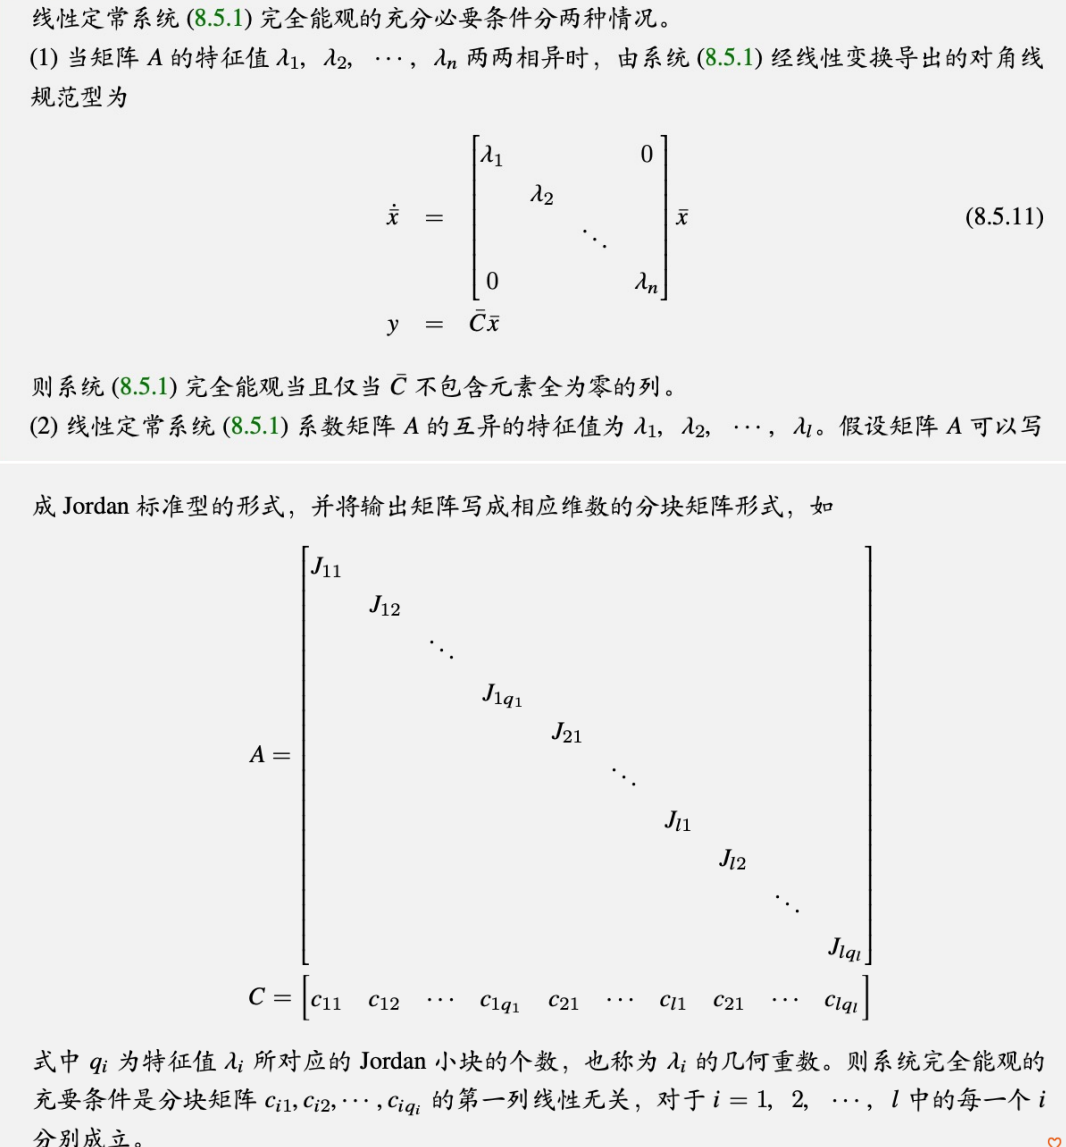
\includegraphics[width = .7\textwidth]{note/state space/figure/17.png}
    \end{center}
\end{theorem}

\subsection{连续系统结构分解}

\subsubsection{对偶性原理}
从上述能控性和能观性的定理和定义中可以看到，这两个概念是非常相似的，这两个概念在数学上是对称的，存在对偶性，我们可以通过下面的表为例：

\begin{center}
    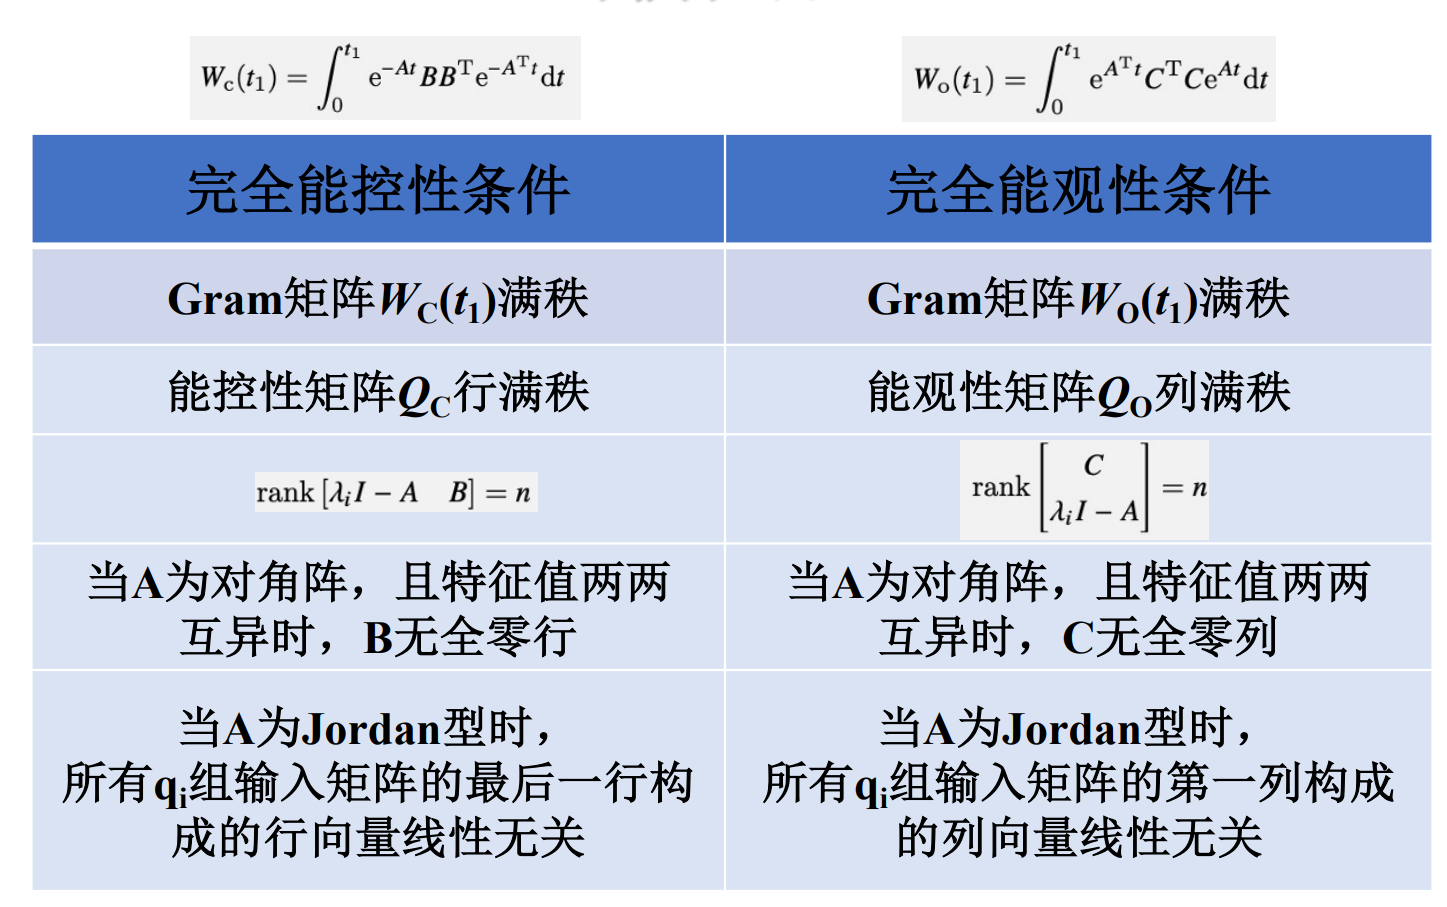
\includegraphics[width = .6\textwidth]{note/state space/figure/18.png}
\end{center}

\begin{definition}[对偶系统]
    线性定常系统
    \begin{equation*}
        \begin{cases}
            \dot{x} = A x + B u \\
            y = C x
        \end{cases}
    \end{equation*}
    的对偶系统为：
    \begin{equation*}
        \begin{cases}
            \dot{z} = A^T z + C^T v\\
            w = B^T z
        \end{cases}
    \end{equation*}

    由对偶性可以知道，如果原系统完全能控，则对偶系统完全能观；如果原系统完全能观，则对偶系统完全能控
\end{definition}

\subsubsection{能控规范型}

以下部分讨论的都是单输入单输出系统：
\begin{equation*}
    \begin{cases}
        \dot{x} = A x + b u \\
        y = C x
    \end{cases}
\end{equation*}
系统的特征多项式为：$\sum\limits_{i=0}^n \alpha_i s^i$，其中$\alpha_n = 1$，其能控性矩阵为:$Q_c = [
    \begin{array}{cccc}
        Ab & A^2 b & \cdots & A^{n-1} b
    \end{array}
]$

\begin{theorem}[第一能控性规范型]
    给定单输入单输出能控性系统，则在状态变换$x = Q_c \bar{x}$下，系统可转换为如下的第一能控规范型：
    \begin{equation*}
        \begin{cases}
            \dot{\bar{x}} = A_c \bar{x} + b_c u \\
            y = C_c \bar{x}
        \end{cases}
    \end{equation*}

    其中：
    \begin{equation*}
        \begin{split}
            A_c =  \begin{bmatrix}
            0 & \cdots & 0 & -\alpha_0 \\
            1 & \cdots & 0 & -\alpha_1 \\
              & \ddots & \vdots & \cdots \\
              & & 1 & -\alpha_{n-1} \\
        \end{bmatrix} , b_c = \begin{bmatrix}
            1 \\ 0 \\ \vdots \\ 0
        \end{bmatrix}  \\
        c_c = cQ_c = \begin{bmatrix}
            \beta_0 & \beta_1 & \cdots & \beta_{n-1} \\
        \end{bmatrix}\\
        \end{split}
    \end{equation*}
    \begin{equation*}
        \beta_i = c A^i b \quad \forall i < n
    \end{equation*}
\end{theorem}

\begin{theorem}[第二能控性规范型]
    给定单输入单输出能控性系统，其由特征多项式系数构成的Hankel矩阵$H_A$为：
    \begin{gather*}
        H_A = \begin{bmatrix}
            \alpha_1     & \alpha_2 & \cdots & \alpha_{n-1}  & 1       \\
            \alpha_2     & \alpha_3 & \cdots & 1             & 0       \\
            \vdots       & \vdots   & \ddots & \vdots        & \vdots  \\
            \alpha_{n-1} & 1        & \cdots & 0             & 0       \\
            1            & 0        & \cdots & 0             & 0       \\
        \end{bmatrix}
    \end{gather*}
    设其能控性矩阵为$Q_C$。令$P = Q_C H_A$，在状态变换$x = P \bar{x}$下，系统可转换为如下的第二能控规范型：
    \begin{equation*}
        \begin{cases}
            \dot{\bar{x}} = A_c \bar{x} + b_c u \\
            y = C_c \bar{x}
        \end{cases}
    \end{equation*}
    其中：
    \begin{gather*}
        A_C = \begin{bmatrix}
            0 & 1 & \cdots & 0 \\
            \vdots & \vdots &  & \vdots \\
            0 & 0 & \cdots & 1 \\
            -\alpha_0 & -\alpha_1 & \cdots & -\alpha_{n-1}
        \end{bmatrix} , \,
        b_c = \begin{bmatrix}
            0 & 0 & \cdots & 1 \\
        \end{bmatrix}^T  \\
        C_c = C P = \begin{bmatrix}
            \beta_0 & \beta_1 &  \cdots & \beta_{n-1}
        \end{bmatrix} \text{其中：}
        \begin{cases}
            \beta_{n-1} = C b \\
            \beta_{n-2} = C A b + \alpha_{n-1} C b \\
            \vdots \\
            \beta_1 = C A^{n-2} b + \alpha_{n-1} C A^{n-3} b + \cdots + \alpha_2 C b \\
            \beta_0 = C A^{n-1} b + \alpha_{n-1} C A^{n-2} b + \cdots + \alpha_1 C b \\
        \end{cases}
    \end{gather*}

    由第二能控标准型我们可以直接写出系统的闭环传递函数：
    \begin{gather*}
        D(s) = \frac{\sum\limits_{i=0}^{n-1} \beta_i s^i}{s^n + \sum\limits_{j=1}^{n-1} \alpha_i s^i}
    \end{gather*}
\end{theorem}

\subsubsection{能观规范型}

和能控规范型类似，以下部分讨论的都是单输入单输出系统：
\begin{equation*}
    \begin{cases}
        \dot{x} = A x + b u \\
        y = C x
    \end{cases}
\end{equation*}
系统的特征多项式为：$\sum\limits_{i=0}^n \alpha_i s^i$，其中$\alpha_n = 1$，其能观性矩阵为：$Q_O = \begin{bmatrix}
    C^T & A^T C^T & \cdots (A^T)^{n-1} C^T \\
\end{bmatrix}^T$

\begin{theorem}[第一能观规范型]
    给定单输入单输出能观性系统，则在状态变换$x = Q_O^{-1} \tilde{x}$下，系统可转换为如下第一能观规范型
    \begin{gather*}
        \dot{\tilde{x}} = \begin{bmatrix}
            0 & 1 & \cdots & 0 \\
            \vdots & \vdots & & \vdots \\
            0 & 0 & \cdots & 1 \\
            -\alpha_0 & -\alpha_1 &  \cdots & -\alpha_{n-1}
        \end{bmatrix} \tilde{x} + \begin{bmatrix}
            \beta_0 \\ \beta_1 \\ \vdots \\ \beta_{n-1}
        \end{bmatrix} u \\
        y = \begin{bmatrix}
            1 & 0 & \cdots & 0
        \end{bmatrix} \tilde{x}
    \end{gather*}

    其中：
    \begin{gather*}
        \beta_i = C A^i b\\
        b_O = Q_O b = \begin{bmatrix}
            \beta_0 \\ \beta_1 \\ \vdots \\ \beta_{n-1}
        \end{bmatrix}
    \end{gather*}
\end{theorem}

\begin{theorem}[第二能观规范型]
    给定单输入单输出能观性系统，其对应的Hankel矩阵为：
    \begin{gather*}
        H_A = \begin{bmatrix}
            \alpha_1     & \alpha_2 & \cdots & \alpha_{n-1}  & 1       \\
            \alpha_2     & \alpha_3 & \cdots & 1             & 0       \\
            \vdots       & \vdots   & \ddots & \vdots        & \vdots  \\
            \alpha_{n-1} & 1        & \cdots & 0             & 0       \\
            1            & 0        & \cdots & 0             & 0       \\
        \end{bmatrix}
    \end{gather*}
    令$Q = H_A Q_O$则在状态变换$x = Q^{-1} \tilde{x}$下，系统可转换为如下第二能观规范型：
    \begin{gather*}
        \dot{\tilde{x}} = \begin{bmatrix}
            0 & \cdots & 0 & -\alpha_0 \\
            1 & \cdots & 0 & -\alpha_1 \\
            \vdots & & \vdots & \vdots \\
            0 & \cdots & 1 & -\alpha_{n-1} 
        \end{bmatrix} \tilde{x} + \begin{bmatrix}
            \beta_0 \\ \beta_1 \\ \vdots \\ \beta_{n-1} \\
        \end{bmatrix} u  \\
        y = \begin{bmatrix}
            0 & \cdots & 0 & 1
        \end{bmatrix} \tilde{x}
    \end{gather*}
    其中：
    \begin{gather*}
        \begin{cases}
            \beta_{n-1} = C b \\
            \beta_{n-2} = C A b + \alpha_{n-1} C b \\
            \vdots \\
            \beta_1 = C A^{n-2} b + \alpha_{n-1} C A^{n-3} b + \cdots + \alpha_2 C b \\
            \beta_0 = C A^{n-1} b + \alpha_{n-1} C A^{n-2} b + \cdots + \alpha_1 C b 
        \end{cases}
    \end{gather*}
\end{theorem}

\subsubsection{能控性结构分解}

但是对于一个不完全能控的系统，其无法化为能控标准型，我们这时候应当如何提取出其中的能控部分，将能控部分和不能控部分分开呢？我们有以下的方式：

\begin{anymark}[能控性结构分解]
    给定一个$n$维线性定常系统，其能控性矩阵为$Q_C$，且有$\text{rank} Q_C < n$。$l_1 , l_2 , \cdots ,l_k$是$Q_C$列空间中$k$个线性无关的列向量，$l_{k+1},\cdots,l_n$是与向量组$\{l_1,l_2,\cdots,l_k\}$线性无关的$(n-k)$个线性无关的列向量，并令变换矩阵$P = \begin{bmatrix}
        l_1 & l_2 & \cdots & l_k & l_{k+1} & \cdots & l_n 
    \end{bmatrix}$。则状态变换$x = P \hat{x}$可将系统转化为按能控性分解的规范形式：
    \begin{gather*}
        \begin{cases}
            \begin{bmatrix}
                \dot{\hat{x}}_C \\ \dot{\hat{x}}_{\bar{C}}
            \end{bmatrix} = \begin{bmatrix}
                \hat{A}_C & \hat{A}_{12} \\
                0         & \hat{A}_{\bar{C}}\\
            \end{bmatrix} \begin{bmatrix}
                \hat{x}_C \\ \hat{x}_{\bar{C}}
            \end{bmatrix} + \begin{bmatrix}
                \hat{B}_C \\ 0
            \end{bmatrix} u \\
            y = \begin{bmatrix}
                \hat{C}_1 & \hat{C}_2
            \end{bmatrix} \begin{bmatrix}
                \hat{x}_C  \\  \hat{x}_{\bar{C}}
            \end{bmatrix}
        \end{cases}
    \end{gather*}
    并且有如下的结论成立：
    \begin{enumerate}
        \item $(\hat{A}_C,\hat{B}_C)$是完全能控的
        \item 子系统$\Sigma(\hat{A}_C,\hat{B}_C,\hat{C}_1)$的传递函数等于整个系统的传递函数，即：
        \begin{gather*}
            \hat{C}_1 (sI - \hat{A}_C)^{-1} \hat{B}_C = C (sI - A)^{-1} B
        \end{gather*}
        \item 两个子系统$\Sigma_1(\hat{A}_C,\hat{B}_C,\hat{C}_1),\Sigma_2(\hat{A}_{\bar{C}},\hat{B}_{\bar{C}},\hat{C}_2)$的特征多项式的乘积等于原系统的特征多项式\\
        其中两个子系统为：
        \begin{equation*}
            \begin{split}
                &\Sigma_1:\begin{cases}
                \dot{\hat{x}}_C = \hat{A}_C \hat{x}_C + \hat{A}_{12} \hat{x}_{\bar{C}} + \hat{B}_C u\\
                y_1 = \hat{C}_1 \hat{x}_C
                \end{cases} \\
                &\Sigma_2:\begin{cases}
                    \dot{\hat{x}}_{\bar{C}} = \hat{A}_{\bar{C}} \hat{x}_{\bar{C}} \\
                    y_2 = \hat{C}_2 \hat{x}_{\bar{C}}
                \end{cases}
            \end{split}
        \end{equation*}
        $\Sigma_1$为$k$维完全能控的子系统，$\Sigma_2$为$n-k$维不能控子系统，$y = y_1 + y_2$
    \end{enumerate}
    \begin{marker}
        对于一个不完全可控的系统，其能控性结构分解是不唯一的，因为不同的人取的$n$个线性无关的列向量不完全一样，导致变换矩阵$P$不相同
    \end{marker}
\end{anymark}

\subsubsection{能观性结构分解}

和上面类似，我们可以通过以下的方式将系统中的能观部分和不能观部分分开：
\begin{anymark}[能观性结构分解]
    给定$n$维线性定常系统，其能观性矩阵为$Q_o$，且有$\text{rank} Q_o = k < n$。$v_1^T,v_2^T,\cdots,v_k^T$是$Q_o$行空间中$k$个线性无关的行向量，$v_{k+1}^T,\cdots,v_n^T$是与向量组$\{v_1^T,v_2^T,\cdots,v_k^T\}$线性无关的$(n-k)$个线性无关的行向量，并令变换矩阵$P = \begin{bmatrix}
        v_1^T \\ v_2^T \\ \vdots \\ v_n^T
    \end{bmatrix}^T$，则线性变换$x = P^{-1} \hat{x}$将上述系统化为按能观性分解的规范型
    \begin{gather*}
        \begin{cases}
            \begin{bmatrix}
                \dot{\hat{x}}_o \\ \dot{\hat{x}}_o
            \end{bmatrix} = \begin{bmatrix}
                \hat{A}_o & 0 \\
                \hat{A}_{21} & \hat{A}_{\bar{o}}
            \end{bmatrix} \begin{bmatrix}
                \hat{x}_o \\ \hat{x}_{\bar{o}}
            \end{bmatrix} + \begin{bmatrix}
                \hat{B}_1 \\ \hat{B}_2
            \end{bmatrix} u\\
            y = \begin{bmatrix}
                \hat{C}_o & 0
            \end{bmatrix} \begin{bmatrix}
                \hat{x}_o \\ \hat{x}_{\bar{o}}
            \end{bmatrix}
        \end{cases}
    \end{gather*}
    并且有如下的结论成立：
    \begin{enumerate}
        \item $(\hat{A}_o, \hat{C}_o)$完全能观
        \item 子系统$\Sigma(\hat{A}_o,\hat{B}_1,\hat{C}_o)$的传递函数等于整个系统的传递函数，即：
        \begin{gather*}
            \hat{C}_o (sI - \hat{A}_o)^{-1} \hat{B}_1 = C (sI - A)^{-1} B
        \end{gather*}
        \item 两个子系统$\Sigma_1(\hat{A}_C,\hat{B}_C,\hat{C}_1),\Sigma_2(\hat{A}_{\bar{C}},\hat{B}_{\bar{C}},\hat{C}_2)$的特征多项式的乘积等于原系统的特征多项式\\
        其中两个子系统为：
        \begin{equation*}
            \begin{split}
                &\Sigma_1:\begin{cases}
                \dot{\hat{x}}_o = \hat{A}_o \hat{x}_o + \hat{B}_1 u\\
                y_1 = \hat{C}_o \hat{x}_o
                \end{cases} \\
                &\Sigma_2:\begin{cases}
                    \dot{\hat{x}}_{\bar{o}} = \hat{A}_{21} \hat{x}_o + \hat{A}_{\bar{o}} \hat{x}_{\bar{o}} + \hat{B}_2 u \\
                    y_2 = 0
                \end{cases}
            \end{split}
        \end{equation*}
        $\Sigma_1$为$k$维完全能观的子系统，$\Sigma_2$为$n-k$维不能观子系统，$y = y_1 + y_2$
    \end{enumerate}
\end{anymark}

\subsubsection{能控+能观结构分解}

此处考试不做要求，下面仅给出课上的ppt：
\begin{center}
    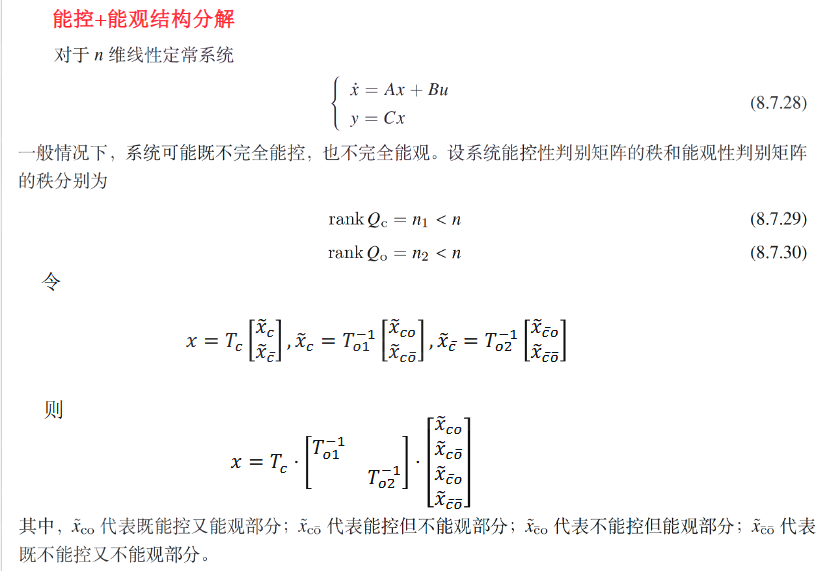
\includegraphics[width = .8\textwidth]{note/state space/figure/19.png} \\
    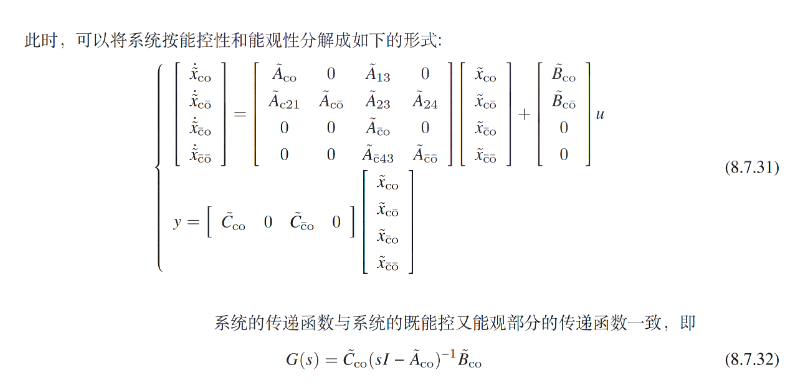
\includegraphics[width = .8\textwidth]{note/state space/figure/20.png}
\end{center}

\subsection{状态空间实现}

\subsubsection{能控能观性与零极点对消}

对于SISO系统，如果要通过秩判据一步一步判别系统的能控能观性，花费的精力会比较大，如果系统既是能控的也是能观的，我们有没有什么比较快的方法呢？

当然有！我们通过以下的定理来判别系统的能控能观性：
\begin{theorem}
    对于单输入单输出系统，一个传递函数的实现是能控能观的当且仅当传递函数无零极点对消
    \begin{marker}
        传递函数的实现指的是可以化成该传递函数的状态空间模型，注意在化成传递函数的过程中不要轻易约去分子分母的公因式！
    \end{marker}
\end{theorem}

\subsubsection{单输入单输出系统的实现}

对于一个单输入单输出系统，已知系统的传递函数，如果系统传递函数没有零极点对消，我们可以：
\begin{enumerate}
    \item 建立系统的能控规范型实现
    \item 建立系统的能观规范型实现
    \item 通过传递函数的部分分式展开，写出系统的Jordan标准型的实现形式
\end{enumerate}

\subsubsection{最小实现}

对于给定的传递函数矩阵，其实现并不唯一，其中维数最小的实现被称为最小实现。因此，最小实现是一种结构最简单的不可约实现。关于线性定常系统的最小实现有如下定理：
\begin{theorem}
    $G(s)$是一个严格真有理分实矩阵，实现$\Sigma(A,B,C)$是它最小实现的充要条件为：$(A,B)$能控，$(A,C)$能观  
\end{theorem}

\begin{theorem}
    $G(s)$任意两个最小实现$\Sigma_1(A_1,B_1,C_1)$和$\Sigma_2(A_2,B_2,C_2)$是代数等价的
\end{theorem}

那么怎么寻找最小实现呢？我们有以下的方式：
\begin{enumerate}
    \item 根据给定的传递函数矩阵$G(s)$，首先找出一种实现，为了使实现具有较低的维数，通常的做法是，当输入维数小于输出维数时，选择能控标准型实现，反之，选择能观标准型实现
    \item 对这个实现进行结构分解，其中既能控又能观的部分便是最小实现
\end{enumerate}


\begin{theorem}[能控标准型实现]
    模型
    \begin{equation*}
        \begin{cases}
            \dot{x} = Ax + Bu \\
            y = Cx
        \end{cases}
    \end{equation*}
    作为给定传递矩阵$ G(s) = \dfrac{\sum\limits_{i=0}^{n-1} P_i s^i}{s^n + \sum\limits_{j=0}^{n-1} \alpha_i s^i}$的一个能控标准型实现为
    \begin{equation*}
    \begin{cases}
        A = \begin{bmatrix}
        0_r & I_r & 0_r & \cdots & 0_r \\
        0_r & 0_r & I_r & \cdots & 0_r \\
        \vdots & \vdots & \vdots & & \vdots \\
        0_r & 0_r & 0_r & \cdots & I_r \\
        -\alpha_0 I_r & -\alpha_1 I_r & -\alpha_2 I_r & \cdots & -\alpha_{n-1} I_r
        \end{bmatrix} \in \mathbb{R}^{rn \times rn}
        \\[20pt]
        B = \begin{bmatrix}
        0_r \\
        0_r \\
        \vdots \\
        0_r \\
        I_r
        \end{bmatrix} \in \mathbb{R}^{rn \times r}
        \\[20pt]
        C = \begin{bmatrix}
        P_0 & P_1 & \cdots & P_{n-1}
        \end{bmatrix} \in \mathbb{R}^{m \times rn}
        \end{cases}
    \end{equation*}
    其中 $0_r$ 及 $I_r$ 分别为 $r \times r$ 零矩阵及 $r \times r$ 单位矩阵。
\end{theorem}


\begin{theorem}[能观标准型实现]
    模型
    \begin{equation*}
        \begin{cases}
            \dot{x} = Ax + Bu \\
            y = Cx
        \end{cases}
    \end{equation*}
    作为给定传递矩阵$ G(s) = \dfrac{\sum\limits_{i=0}^{n-1} P_i s^i}{s^n + \sum\limits_{j=0}^{n-1} \alpha_i s^i}$的一个能观标准型实现为
    \begin{equation*}
        \begin{cases}
        A = \begin{bmatrix}
        0_m & 0_m & \cdots & 0_m & -\alpha_0 I_m \\
        I_m & 0_m & \cdots & 0_m & -\alpha_1 I_m \\
        0_m & I_m & \cdots & 0_m & -\alpha_2 I_m \\
        \vdots & \vdots & & \vdots & \vdots \\
        0_m & 0_m & \cdots & I_m & -\alpha_{n-1} I_m
        \end{bmatrix} \in \mathbb{R}^{mn \times mn}
        \\[20pt]
        B = \begin{bmatrix}
        P_0 \\
        P_1 \\
        \vdots \\
        P_{n-1}
        \end{bmatrix} \in \mathbb{R}^{mn \times r}
        \\[20pt]
        C = \begin{bmatrix}
        0_m & 0_m & \cdots & 0_m & I_m
        \end{bmatrix} \in \mathbb{R}^{m \times mn}
        \end{cases}
    \end{equation*}
    其中 $0_m$ 及 $I_m$ 分别为 $m \times m$ 零矩阵及 $m \times m$ 单位矩阵。
\end{theorem}

\subsection{离散系统能控能观性}

\subsubsection{离散系统能控性}

对于离散系统我们考察以下定常线性离散时间系统的能控性：
\begin{gather*}
    x(k + 1) = G x(k) + H u(k)
\end{gather*}

\begin{definition}[能控状态]
    对于线性定常离散时间系统，如果存在一时刻$k_1 > 0$和一个无约束控制$u(k),k \in \mathbb{I}[0,k_1]$，使得系统在这个控制的作用下，系统由初始状态$x(0) = x_0$出发经过$k_1$步后转移到$x(k_1) = 0$，则称此状态$x_0$是系统的一个能控状态
\end{definition}

\begin{definition}[系统的能控性]
    对于线性定常离散时间系统，如果状态空间中的所有非零状态都是能控状态，则称该系统是能控的
\end{definition}

不过，在线性定常离散时间系统中，系统的能控性和能达性并不等价，我们给出以下的能达性的定义：
\begin{definition}[能达状态]
    对于线性定常离散时间系统，如果存在一时刻$k_1 > 0$，和一个无约束控制$u(k)$，使得系统在这个控制的作用下，系统由零初始状态$x(0) = 0$出发后转移到$x(k_1) = x_f$，则称此$x_f$是系统的一个能达状态
\end{definition}

\begin{definition}[系统能达性]
    对于线性定常离散时间系统，如果状态空间中的所有非零状态都是能达状态，则称该系统是能达的
\end{definition}

和连续系统类似，我们也可以给出离散系统中能控性和能达性的判据：

\begin{anymark}[能控性Gram判据]
    给定输入矩阵$H \in \mathbb{R}^{n \times r }$和非奇异系统矩阵$G \in \mathbb{R}^{n\times n}$，线性定常系统是能控的，当且仅当存在时刻$k_1 > 0$，使得Gram矩阵：
    \begin{gather*}
        W_c(k_1) = \sum_{i=0}^{k_1 - 1} G^{-1-i} H H^T (G^{-1-i})^T
    \end{gather*}
    是非奇异的
\end{anymark}

\begin{anymark}[能达性Gram判据]
    给定输入矩阵$H \in \mathbb{R}^{n \times r }$和非奇异系统矩阵$G \in \mathbb{R}^{n\times n}$，线性定常系统是能达的，当且仅当存在时刻$k_1 > 0$，使得Gram矩阵：
    \begin{gather*}
        W_c(k_1) = \sum_{i=0}^{k_1 -1} G^{k_1-1-i} H H^T (G^{k_1-1-i})^T
    \end{gather*}
    是非奇异的
\end{anymark}

\begin{anymark}[能控性和能达性的秩判据]
    给定输入矩阵$H \in \mathbb{R}^{n \times r }$和系统矩阵$G \in \mathbb{R}^{n\times n}$
    \begin{enumerate}
        \item 系统是\textbf{能达}的，当且仅当：
        \begin{gather*}
            \text{rank} \begin{bmatrix}
                H & GH & \cdots & G^{n-1} H
            \end{bmatrix} = n
        \end{gather*}
        \item 系统是\textbf{能控}的，当且仅当：
        \begin{gather*}
            \text{rank} \begin{bmatrix}
                H & GH & \cdots & G^{n-1} H
            \end{bmatrix} = \text{rank} \begin{bmatrix}
                H & GH & \cdots & G^{n-1} H & G^n
            \end{bmatrix}
        \end{gather*}
    \end{enumerate}
    观察以上两个判据，可以发现两个判据等价的充要条件为：\textbf{系统矩阵$G$是非奇异的}
\end{anymark}

\begin{theorem}[最小拍控制]
    考虑单输入离散时间线性时不变系统：
    \begin{equation*}
        x(k+1) = Gx(k) + hu(k), \quad k = 0, 1, \cdots
    \end{equation*}
    其中，$x$ 为 $n$ 维状态，$u$ 为标量输入，$G$ 和 $h$ 为 $n \times n$ 和 $n \times 1$ 常值矩阵，且设 $G$ 非奇异，那么，当系统为完全能控时，可构造如下一组控制输入：
    \begin{equation*}
        \begin{bmatrix}
        u(0) \\ u(1) \\ \cdots \\ u(n-1)
        \end{bmatrix}
        = -\bigl[ G^{-1}h,\ G^{-2}h,\ \cdots,\ G^{-n}h \bigr]^{-1} x_0
    \end{equation*}
    使系统必可在 $n$ 步内由任意非零初始状态 $x(0) = x_0$ 转移到状态空间原点。通常称这组控制为\textbf{最小拍控制}。
\end{theorem}

\subsubsection{离散系统能观性}

对于离散系统我们考察以下定常线性离散时间系统的能观性
\begin{gather*}
    \begin{cases}
        x(k+1) = G x(k) \\
        y(k) = C x(k)
    \end{cases}
\end{gather*}

\begin{definition}[能观状态]
    对于线性定常离散时间系统，如果对于初始时刻$k = 0$的一个非零的初始状态$x_0$，存在一个有限的时刻$k_1 > 0$，使得由区间$\mathbb{I}[0,k_1]$上的系统的输出$y(k)$可以唯一决定系统初始状态$x_0$，则称该状态$x_0$是能观的
\end{definition}

\begin{definition}[系统的能观性]
    对于线性定常离散时间系统，如果状态空间中的所有非零状态都是能观状态，则称该系统是能观的
\end{definition}

同样的，我们也可以给出离散系统中能观性判据：
\begin{anymark}[离散系统能观性Gram判据与秩判据]
    给定系统矩阵 $G \in \mathbb{R}^{n \times n}$ 和输出矩阵 $C \in \mathbb{R}^{m \times n}$，线性离散定常系统是能观的，当且仅当
    \begin{enumerate}
        \item \textbf{Gram判据}：存在有限时刻 $k_1 > 0$，使得 Gram 矩阵
        \begin{equation*}
            W_o(k_1) = \sum_{i=0}^{k_1} (G^{\mathrm{T}})^i C^{\mathrm{T}} C G^i
        \end{equation*}
        是非奇异的。
        \item \textbf{秩判据}：
        \begin{equation*}
            \mathrm{rank}\, Q_{od} = \mathrm{rank}
            \begin{bmatrix}
            C \\ CG \\ \vdots \\ CG^{n-1}
            \end{bmatrix} = n
        \end{equation*}
        或
        \begin{equation*}
            \mathrm{rank}
            \begin{bmatrix}
            C^{\mathrm{T}} & G^{\mathrm{T}}C^{\mathrm{T}} & (G^{\mathrm{T}})^2 C^{\mathrm{T}} & \cdots & (G^{\mathrm{T}})^{n-1} C^{\mathrm{T}}
            \end{bmatrix} = n
        \end{equation*}
    \end{enumerate}
\end{anymark}

\begin{theorem}[最小拍观测]
    考虑单输出离散时间线性时不变系统：
    \begin{align*}
        x(k+1) &= Gx(k), \quad x(0) = x_0, \quad k = 0, 1, 2, \cdots \\
        y(k) &= cx(k)
    \end{align*}
    其中 $x \in \mathbb{R}^n$，$y \in \mathbb{R}$，$G \in \mathbb{R}^{n \times n}$，$c \in \mathbb{R}^{1 \times n}$。那么，若系统完全能观测，则只利用 $n$ 步输出值 $y(0), y(1), \cdots, y(n-1)$ 就可构造相应初始状态 $x_0$：
    \begin{equation*}
        x_0 =
        \begin{bmatrix}
        c \\ cG \\ \vdots \\ cG^{n-1}
        \end{bmatrix}^{-1}
        \begin{bmatrix}
        y(0) \\ y(1) \\ \vdots \\ y(n-1)
        \end{bmatrix}
    \end{equation*}
\end{theorem}

\subsubsection{离散化系统对能控能观性的保持}

\begin{proposition}
    如果连续系统是不完全可控（不完全可观），则其离散化系统也是不能控（不能观）的
    \begin{proof}
        如果线性定常连续系统不能控，则其能控性矩阵
        \begin{equation*}
            Q_c = \begin{bmatrix} B & AB & \cdots & A^{n-1}B \end{bmatrix}
        \end{equation*}
        秩为 $\mathrm{rank}\,Q_c = k < n$，设列向量 $l_1, l_2, \ldots, l_k$ 是 $Q_c$ 中线性无关的列。

        对离散化系统，其能控性矩阵为：
        \begin{equation*}
            Q_{cd} = \begin{bmatrix} H & GH & \cdots & G^{n-1}H \end{bmatrix}
        \end{equation*}
        其中 $G = e^{AT},\ H = \left(\displaystyle\int_0^T e^{A\tau} d\tau\right) B$。

        通过 Cayley-Hamilton 定理：
        \begin{itemize}
            \item $\int_0^T e^{A\tau} d\tau$ 可表示为 $\{I, A, \cdots, A^{n-1}\}$ 的线性组合；
            \item 故 $H$ 可表示为 $\{B, AB, \cdots, A^{n-1}B\}$ 的线性组合；
            \item 进而 $H$ 的每列均可表示为 $l_1, l_2, \ldots, l_k$ 的线性组合。
        \end{itemize}

        对于 $GH$：
        \begin{equation*}
            GH = e^{AT} \int_0^T e^{At} B \,dt = \int_0^T e^{A(t+T)} B \,dt
        \end{equation*}

        同样通过 Cayley-Hamilton 可得：
        \begin{itemize}
            \item $GH$ 是 $\{B, AB, \cdots, A^{n-1}B\}$ 的线性组合；
            \item 所以 $GH$ 的每一列也可表示为 $l_1, l_2, \ldots, l_k$ 的线性组合。
        \end{itemize}

        类似地，所有 $G^{i-1}H$ 的每列也都可表示为这些列向量的线性组合。

        结论：
        \begin{equation*}
            \mathrm{rank}\,Q_{cd} \le k < n
        \end{equation*}
        即：离散化系统仍然不可控。对能观性也可以得出类似结论。

    \end{proof}
\end{proposition}

\begin{theorem}
    设系统
    \begin{gather*}
        \Sigma:\begin{cases}
            \dot{x} = A x + B u \quad x(0) = x_0 \\
            y = C x + D u \quad t \geq 0
        \end{cases}
    \end{gather*}
    能控或能观，令 $\lambda_1, \lambda_2, \cdots, \lambda_\mu$ 为 $A$ 的全部特征值，且当 $i \neq j$ 时有 $\lambda_i \neq \lambda_j$，则时间离散化系统 $\Sigma_T$ 保持能控或能观测的一个充分条件是，采样周期 $T$ 的数值对一切满足
    \begin{equation*}
        \mathrm{Re}|\lambda_i - \lambda_j| = 0 \qquad i, j = 1, 2, \cdots, \mu
    \end{equation*}
    的特征值，有
    \begin{equation*}
        T \neq \frac{2l\pi}{\mathrm{Im}(\lambda_i - \lambda_j)} \qquad l = \pm 1, \pm 2, \cdots
    \end{equation*}
\end{theorem}